\chapter{Learning a metric for clustering}\label{chap:clustering-metric}
In section \ref{sec:mil-clustering}, a method for learning a representation \( \phi \) was shown. In order to learn the parameters of the representation, a clustering-loss function is required in the form
\[ L_C : \mathcal{P}^M \left( \bar{\mathspace{X}} \right) \to \mathfield{R} \]
In this chapter, three ways of constructing such a clustering-loss function are explored. The chapter is structured as follows: First, an unsupervised method constructing a clustering loss-function is presented, followed by two supervised methods. Each of the methods builds on some prior art, which is introduced first, followed by an explanation of how the prior art was modified to solve the problem at hand.

\section{Contrastive predictive coding}
Contrastive predictive coding is a technique first introduced by \cite{oord_representation_2019}. In this section, the original article is first presented, with its application to MIL clustering introduced subsequently.

\subsection{Original method}
\name{Contrastive predictive coding} (also referred to as \name{CPC}) builds the model on the ideas from predictive coding (see \cite{elias_predictive_1955}), a technique from information theory. In predictive coding, a sequence of messages is transmitted. Both the transmitter and the receiver try to predict future messages from all the past ones. Only the difference between the predicted and actual message is then actually transmitted.

CPC is an approach to representing time series by modelling future data from the past. In order to do that, the model learns high-level representations of the data and discards noise in the data. The further in future the model predicts, the less shared information is available and thus the global structure needs to be inferred better.

First, a non-linear encoder \( g_\mathrm{enc} \) is used to map an input sequence of data to their latent representations:
\[ g_\mathrm{enc} : x_t \mapsto z_t \]
Next, an autoregressive model \( g_\mathrm{ar} \) summarizes all latent representations up to a certain point \( t \) and produces a context latent representation:
\[ c_t = g_\mathrm{ar} \left( \left\{ z_i \middle| i \leq t \right\} \right) \]
Modelling \( p_k \left( x_{t + k} \middle| c_t \right) \) directly using a conditional generative model is computationally very expensive, which is the reason why this approach hasn't been chosen. Instead, the density ratio which preserves the mutual information between \( x_{t + k} \) and \( c_t \) has been modelled as follows:
\begin{equation}\label{equa:CPC-model}
  f_k \left( x_{t + k}, c_t \right) \propto \frac{p \left( x_{t + k} \middle| c_t \right)}{p \left( x_{t + k} \right)}
\end{equation}
A log-bilinear model was used:
\[ f_k \left( x_{t + k}, c_t \right) = \exp \left( z_{t + k}^T W_k c_t \right) \]

Both \( g_\mathrm{enc} \) and \( g_\mathrm{ar} \) have been trained to jointly optimize a loss based on the Noise Contrastive Estimation (see \cite{gutmann_noise-contrastive_2010}), which is called \name{InfoNCE} in \cite{oord_representation_2019}. Given a set \( \mathset{X} = \left\{ x_1, \dots, x_N \right\} \) containing one positive sample from \( p \left( x_{t + k} \middle| c_t \right) \) and \( N - 1 \) negative samples from \( p \left( x_{t + k} \right) \), the InfoNCE loss is as follows:
\[ L_N = - \underset{\mathset{X}}{\mathbb{E}} \left[ \log f_k \left( x_{t + k}, c_t \right) - \log \sum_{x_j \in \mathset{X}} f_k \left( x_j, c_t \right) \right] \]
Optimizing \( L_N \) will result in \( f_k \) estimating the density ratio from equation \ref{equa:CPC-model}.

The model is illustrated in figure \ref{fig:CPC-paper-model}.

\begin{figure}[h]
	\centering
	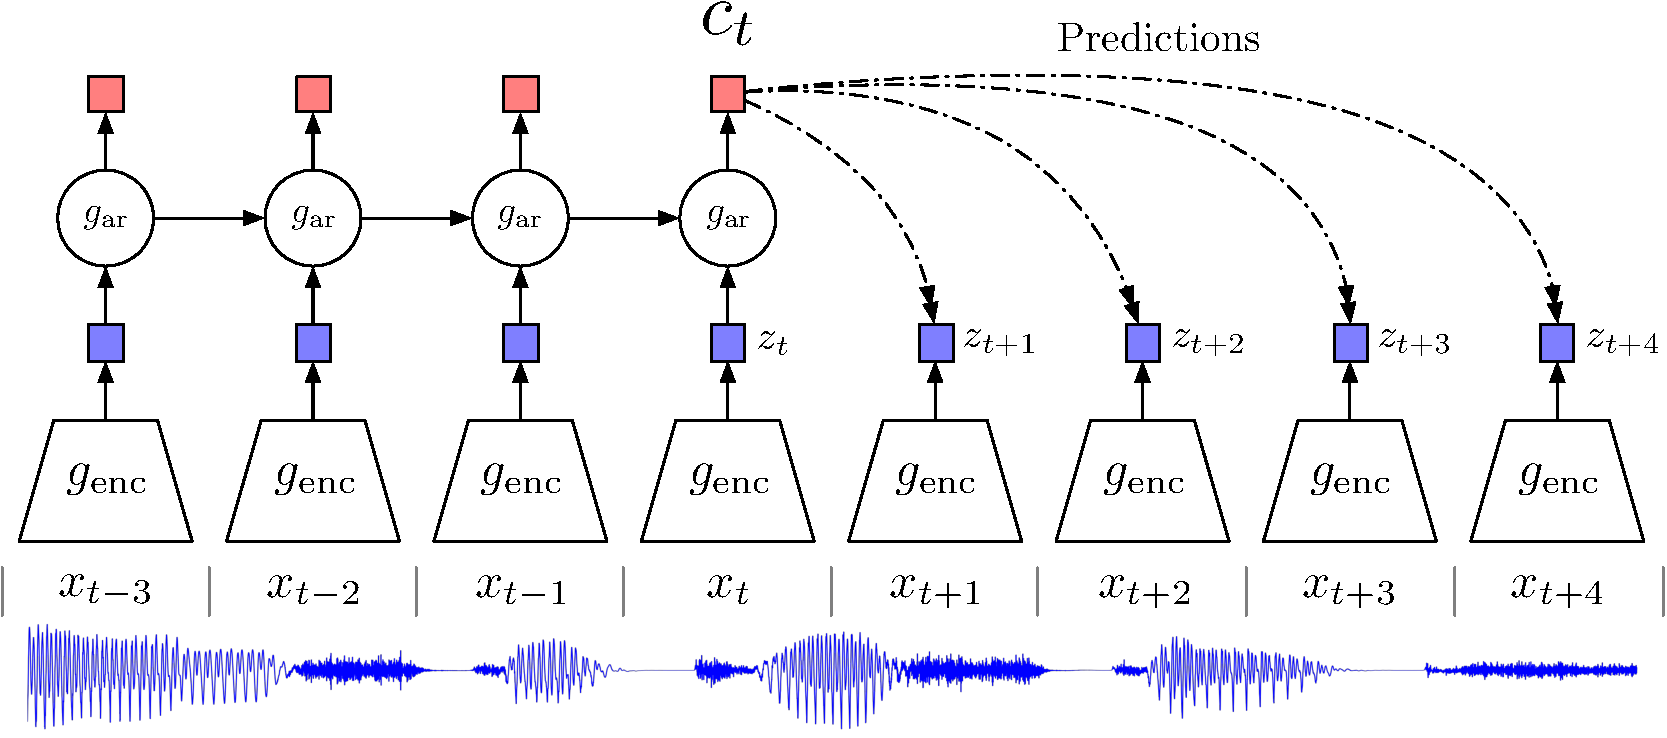
\includegraphics[width=0.9\textwidth]{images/CPC-paper-model.pdf}
	\caption{The Contrastive Predictive Coding model. Image from \cite{oord_representation_2019}}\label{fig:CPC-paper-model}
\end{figure}

\subsection{Application to MIL}\label{subsec:CPC-application}

The core idea taken from CPC to this work is that of the InfoNCE loss. The actual application is based on the following idea. If a bag is split into two parts, it is reasonable to expect that the representations of these two parts would be close to one another. On the other hand, if a random bag were to be drawn from the data (as a \textit{simple random sample with replacement}), it is reasonable to expect it to be relatively far from any actual bag present in the data. These assumptions can be proven correct by using the stochastic formalism for MIL (see section \ref{sec:stochastic-formalism}). Given that each bag \( B_k \) is viewed as a set of realizations of a probability distribution \( P_k \in \mathcal{P}^\mathspace{X} \), it follows that the two parts of the bag, \( B_k^{(1)} \) and \( B_k^{(2)} \) are sets of realizations from the same distribution \( P_k \) and therefore should be statistically indistinguishable. On the other hand, a randomly sampled bag \( B'_j \) does not share the same probability distribution.
Using these assumptions, the following clustering loss is constructed:

\[ B_k^{(1)} \oplus B_k^{(2)} = B_k \in \mathspace{B} \]
\[ \forall j \; B'_j \text{ is a bag of randomly sampled instances from } \mathspace{X} \]
\[ L_\mathrm{CPC} = \log \left\lVert \phi \left( B_k^{(1)} \right) - \phi \left( B_k^{(2)} \right) \right\rVert^2 - \log \sum_{j = 1}^K \left\lVert \phi \left( B_k^{(1)} \right) - \phi \left( B'_j \right) \right\rVert^2 \]
where \( \oplus \) is the multiset sum (see definition \ref{def:multiset-sum}). The first term of the loss function depicts the notion that the representations of the two parts of the bag should be close to one another and corresponds to the first term of InfoNCE, which maximizes the prediction of a matching future sample from the current context. The second term depicts the notion that a random bag should be far from all the bags\footnote{On the off-chance a random bag would be close to \( B_k^{(1)} \), this would be outweighed by the other terms.} and corresponds to the second term of InfoNCE, which minimizes the prediction of a random sample from the current context. Choosing to only use the first part of the bag in the second term has no effect as the two parts are chosen randomly. The value \( K \in \mathfield{N} \) is a hyper-parameter of this method.

This method can be further modified to make it less computationally complex. In order to not have to draw a lot of random bags, it can be reasonably expected that, on average, the representations of two parts of two mismatched bags \( B_{k_1}^{(1)} \) and \( B_{k_2}^{(2)} \) should be far apart. The matrix \( \mathmat{D} \) is constructed as
\[ \mathmat{D}_{ij} = \left\lVert \phi \left( B_i^{(1)} \right) - \phi \left( B_j^{(2)} \right) \right\rVert_2^2 \]
The distances of the corresponding halves are found on the diagonal of \( \mathmat{D} \), whereas the distances of mismatched halves are in the rest of the matrix. Under this assumption the final loss for the CPC method is
\[ L_\mathrm{CPC} = \frac{1}{n} \sum_{i = 1}^n \left( \log \left( \mathmat{D}_{ii} \right) - \log \sum_{\substack{j = 1 \\ j \neq i}}^n \mathmat{D}_{ij} \right) \]
where \( n \) is the number of bags.

\section{Triplet loss}
Triplet loss is a much more direct approach based on \cite{weinberger_distance_2006}. In this section, the original article is first presented, with its application to MIL clustering introduced subsequently.

\subsection{Original method}
The performance of the \( k \)-nearest neighbour algorithm depends heavily on the distance metric used. Typically, the Euclidean distance is used. However, ideally, the metric would adapt to the problem at hand. \cite{weinberger_distance_2006} present a way to learn a Mahalanobis distance metric for kNN such that it has the \textit{homogeneity} and \textit{separation} properties of clustering.

Let \( \left\{ \left( \mathvec{x}_i, y_i \right) \right\}_{i = 1}^n \) be a training dataset with \( \mathvec{x}_i \in \mathfield{R}^d \) and \( y_i \) discrete class labels. The goal is to learn a linear transformation
\[ \mathvec{L} : \mathfield{R}^d \to \mathfield{R}^d \]
This linear transformation is then used to compute squared distances as
\[ \mathcal{D} \left( \mathvec{x}_i, \mathvec{x}_j \right) = \left\lVert \mathvec{L} \left( \mathvec{x}_i - \mathvec{x}_j \right) \right\rVert_2^2 \]

A helper matrix \( \mathmat{y} \) is used such that
\[ \mathmat{y}_{ij} = \begin{cases}
    0 &\text{for} \quad y_i \neq y_j \\
    1 &\text{for} \quad y_i = y_j \\
  \end{cases} \]
In addition to this, for each input \( \mathvec{x}_i \), \( k \) target neighbours are defined that are supposed to be close to \( \mathvec{x}_i \). Euclidean distance may be used to find the target neighbours. A matrix \( \mathmat{\eta} \) is used to indicate target neighbours where \( \mathmat{\eta}_{ij} = 1 \) when \( \mathvec{x}_j \) is a target neighbour of \( \mathvec{x}_i \) and \( 0 \) otherwise.

The cost function features two competing terms. The first term depicts the notion that an input should be close to its target neighbours. The second term depicts the notion that inputs of a different class should be far from one another. The loss is of the form
\[ \varepsilon \left( \mathvec{L} \right) = \sum_{i, j = 1}^n \mathmat{\eta}_{ij} \left\lVert \mathvec{L} \left( \mathvec{x}_i - \mathvec{x}_j \right) \right\rVert_2^2 + c \sum_{i, j, l = 1}^n \mathmat{\eta}_{ij} \left( 1 - \mathmat{y}_{il} \right) \left\{ \left\lVert \mathvec{L} \left( \mathvec{x}_i - \mathvec{x}_l \right) \right\rVert_2^2 - \left\lVert \mathvec{L} \left( \mathvec{x}_i - \mathvec{x}_j \right) \right\rVert_2^2 \right\}_+ \]
where \( c > 0 \) is a hyper-parameter of this method and \( \left\{ \cdot \right\}_+ \) is the hinge loss, i.e.
\[ \left\{ x \right\}_+ = \max \left( 0, 1 - x \right) \]

The loss can be reformulated as an instance of semidefinite programming (see \cite{vandenberghe_semidefinite_1996}). This requires the distance \( \mathcal{D} \) to be reformulated as
\[ \mathcal{D} \left( \mathvec{x}_i, \mathvec{x}_j \right) = \left( \mathvec{x}_i - \mathvec{x}_j \right)^\top \mathvec{M} \left( \mathvec{x}_i - \mathvec{x}_j \right) \]
\[ \mathvec{M} = \mathvec{L}^\top \mathvec{L} \]
This makes it clear that \( \mathcal{D} \) truly is a Mahalanobis distance measure. The hinge loss is replaced by introducing slack variables \( \xi_{ij} \) for all \( i \), \( j \) such that \( \mathmat{y}_{ij} = 0 \). The resulting semidefinite program is: \\

\noindent \textbf{Minimize} \( \displaystyle \sum_{i, j = 1}^n \mathmat{\eta}_{ij} \left( \mathvec{x}_i - \mathvec{x}_j \right)^\top \mathvec{M} \left( \mathvec{x}_i - \mathvec{x}_j \right) + c \sum_{i, j, l = 1}^n \mathmat{\eta}_{ij} \left( 1 - \mathmat{y}_{il} \right) \xi_{ijl} \) \textbf{subject to:}
\begin{enumerate}[\textbf{(\theenumi)}]
  \item \( \displaystyle \left( \mathvec{x}_i - \mathvec{x}_l \right)^\top \mathvec{M} \left( \mathvec{x}_i - \mathvec{x}_l \right) - \left( \mathvec{x}_i - \mathvec{x}_j \right)^\top \mathvec{M} \left( \mathvec{x}_i - \mathvec{x}_j \right) \geq 1 - \xi_{ijl} \)
  \item \( \displaystyle \xi_{ijl} \geq 0 \)
  \item \( \displaystyle \mathvec{M} \) is positive semidefinite
\end{enumerate}

While this program can be solved by standard general-purpose solvers, \cite{weinberger_distance_2006} use a custom solver.

\subsection{Application to MIL}
The idea taken from \cite{weinberger_distance_2006} is the triplet loss itself as the optimizations using semidefinite programming are not of interest for this work.

The matrix \( \mathmat{y} \) is defined the same way as in the original article:
\[ \mathmat{y}_{ij} = \begin{cases}
    0 &\text{for} \quad y_i \neq y_j \\
    1 &\text{for} \quad y_i = y_j \\
  \end{cases} \]
This makes triplet loss a supervised method. The matrix \( \mathmat{\eta} \) can be defined similarly:
\[ \mathmat{\eta}_{ij} = \begin{cases}
    1 &\text{if bag } B_j \text{ is a target neighbour for the bag } B_i \\
    0 &\text{otherwise}
  \end{cases} \]
Next, the pair-wise distance matrix \( \mathmat{D} \) is used, in the same form as in section \ref{subsec:CPC-application}:
\[ \mathmat{D}_{ij} = \left\lVert \phi \left( B_i^{(1)} \right) - \phi \left( B_j^{(2)} \right) \right\rVert_2^2 \]
The loss itself is then expressed as:
\[ L_\mathrm{triplet} = \sum_{ij} \eta_{ij} D_{ij} + c \sum_{ijl} \eta_{ij} \left( 1 - y_{il} \right) \left\{ D_{il} - D_{ij} \right\}_+ \]
where \( c > 0 \) is a hyper-parameter of the method. Although \cite{weinberger_distance_2006} suggest finding \( \mathmat{\eta} \) as the \( k \)-nearest neighbours of a data point, in this work, the loss has been simplified by setting \( \mathmat{\eta}_{ij} = \mathmat{y}_{ij} \).

\section{Magnet loss}
Magnet loss is an enhancement of the previously described triplet loss, first introduced by \cite{rippel_metric_2015}. In this section, the original article is first presented, with its application to MIL clustering introduced subsequently.

\subsection{Original method}
The idea of magnet loss builds upon triplet loss. In the case of triplet, the loss function essentially goes over all triplets of a data point, its target neighbour and a point from a different class and optimizes their distances (hence the name "triplet loss"). Magnet loss instead maintains an explicit model of the distributions of different classes in the representation space. To capture the distributions, the model uses simple clustering models for each class. In the case of the triplet loss, the target neighbourhood is set \textit{a priori} and in the original input space -- but using distances in the original input space is exactly what triplet loss and magnet loss aim to circumvent. To this end, magnet loss uses similarity in the space of representations and updates it periodically. Magnet loss also pursues local separation instead of a global one -- representations of different classes should be separated, but can be interleaved. The difference between triplet loss and magnet loss is visualized in figure \ref{fig:triplet-magnet-difference}.

\begin{figure}[h]
  \centering
  \begin{subfigure}[b]{0.245\textwidth}
    \centering
    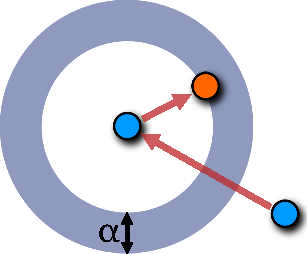
\includegraphics[width=\textwidth]{images/triplet-magnet-difference/triplet_before.pdf}
    \caption{Triplet loss: before}
  \end{subfigure}
  \hfill
  \begin{subfigure}[b]{0.245\textwidth}
    \centering
    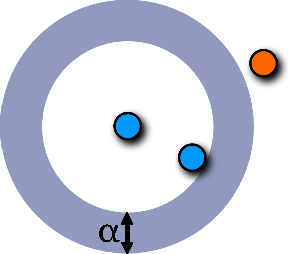
\includegraphics[width=\textwidth]{images/triplet-magnet-difference/triplet_after.pdf}
    \caption{Triplet loss: after}
  \end{subfigure}
  \hfill
  \begin{subfigure}[b]{0.245\textwidth}
    \centering
    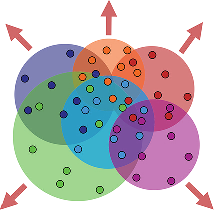
\includegraphics[width=\textwidth]{images/triplet-magnet-difference/magnet_before.pdf}
    \caption{Magnet loss: before}
  \end{subfigure}
  \hfill
  \begin{subfigure}[b]{0.245\textwidth}
    \centering
    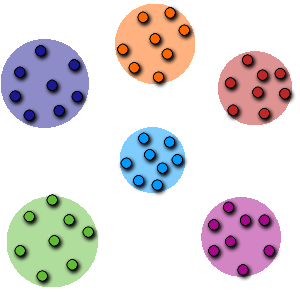
\includegraphics[width=\textwidth]{images/triplet-magnet-difference/magnet_after.pdf}
    \caption{Magnet loss: after}
  \end{subfigure}
  \caption{Visualization of the difference between triplet loss and magnet loss. While triplet loss only considers one data point at a time, magnet loss operates on a neighbourhood of clusters. Image from \cite{rippel_metric_2015}}\label{fig:triplet-magnet-difference}
\end{figure}

Let \( \left\{ \left( \mathvec{x}_i, y_i \right) \right\}_{i = 1}^n \) be a training dataset with inputs \( \mathvec{x}_i \in \mathfield{R}^d \) and \( y_i \) being \( C \) discrete class labels. A general parameterized map \( \mathvec{f} \left( \cdot; \Theta \right) \) embeds the inputs into a representation space:
\[ \mathvec{r}_i = \mathvec{f} \left( \mathvec{x}_i; \Theta \right) \]
For each class \( c \), \( K \) cluster assignments are obtained by using the K-means++ algorithm (see \cite{macqueen_methods_1967} and \cite{arthur_k-means++:_2007}) where \( K \in \mathfield{N} \) is a hyper-parameter of the method:
\[ \mathcal{I}_1^c, \dots, \mathcal{I}_K^c = \argmin_{I_1^c, \dots, I_K^c} \sum_{k = 1}^K \sum_{\mathvec{r} \in I_k^c} \left\lVert \mathvec{r} - \frac{1}{\left\lvert I_k^c \right\rvert} \sum_{\mathvec{r} \in I_k^c} \mathvec{r} \right\rVert_2^2  \]
the centre of each cluster\footnote{\cite{rippel_metric_2015} incorrectly uses \( \mathvec{\mu}_k^c \) as the centre of both \( \mathcal{I}_k^c \) as well as the intermediary cluster \( I_k^c \).} is denoted \( \mathvec{\mu}_k^c \):
\[ \mathvec{\mu}_k^c = \frac{1}{\left\lvert \mathcal{I}_k^c \right\rvert} \sum_{\mathvec{r} \in \mathcal{I}_k^c} \mathvec{r} \]
For each input, the centre of the cluster in which its representation falls is denoted as
\[ \mathvec{\mu} \left( \mathvec{r} \right) = \argmin_{\mathvec{\mu_k^c}} \left\lVert \mathvec{r} - \mathvec{\mu}_k^c \right\rVert \]
and the distance of its representation from the centre of the cluster is denoted as
\[ N_i = \left\lVert \mathvec{r}_i - \mu \left( \mathvec{r}_i \right) \right\rVert_2^2 \]
The variance of the distance of all the representations from their respective centres can then be calculated as
\[ \sigma^2 = \frac{1}{n - 1} \sum_{i = 1}^n N_i \]
For each input, the distance to all the inputs of a different class is calculated as
\[ M_i = \sum_{c \neq y_i} \sum_{k = 1}^K \exp \left( - \frac{1}{2 \sigma^2} \left\lVert \mathvec{r}_i - \mathvec{\mu}_k^c \right\rVert_2^2 \right) \]
The magnet loss is then
\[ L \left( \Theta \right) = \frac{1}{n} \sum_{i = 1}^n \left\{ - \log \frac{\exp \left( - \frac{1}{2 \sigma^2} N_i - \alpha \right)}{M_i} \right\}_+ \]
where \( \alpha \in \mathfield{R} \) is a hyper-parameter of the method, which has the meaning of the desired cluster separation gap with respect to the variance.

This loss function is made computationally less expensive by only sampling a certain amount of clusters for a class, then sampling a certain amount of inputs in each cluster. The rest of the data then isn't considered. This optimization yields the final training procedure:

\begin{enumerate}
  \item Sample a seed cluster \( I_1 \sim p_I \left( \cdot \right) \).
  \item Find the \( M - 1 \) nearest \name{impostor clusters} \( I_2, \dots I_M \) for \( I_1 \).
  \item For each cluster \( I_m \), sample \( D \) examples \( \mathvec{x}_i^m, \dots, \mathvec{x}_D^m \sim p_{I_m} \left( \cdot \right) \).
\end{enumerate}

A stochastic approximation of the loss function is then constructed as
\[ \mathvec{r}_d^m = \mathvec{f} \left( \mathvec{x}_d^m; \Theta \right) \]
\[ \hat{\mathvec{\mu}}_m = \frac{1}{D} \sum_{d = 1}^D \mathvec{r}_d^m \]
\[ \hat{\mathmat{N}}_{md} = \left\lVert \mathvec{r}_d^m - \hat{\mathvec{\mu}}_m \right\rVert_2^2 \]
\[ \hat{\sigma}^2 = \frac{1}{MD - 1} \sum_{m = 1}^M \sum_{d = 1}^D \hat{\mathmat{N}}_{md} \]
\[ \hat{\mathmat{M}}_{md} = \sum_{\substack{\hat{\mathvec{\mu}} \\ C \left( \hat{\mathvec{\mu}} \right) \neq C \left( \mathvec{r}_d^m \right)}} \exp \left( - \frac{1}{2 \hat{\sigma}^2} \left\lVert \mathvec{r}_d^m - \hat{\mathvec{\mu}} \right\rVert_2^2 \right) \]
\[ L \left( \Theta \right) = \frac{1}{MD} \sum_{m = 1}^M \sum_{d = 1}^D \left\{ - \log \frac{\exp \left( - \frac{1}{2 \hat{\sigma}^2} \hat{\mathmat{N}}_{md} - \alpha \right)}{ \hat{\mathmat{M}}_{md} } \right\}_+ \]
where \( C \left( \mathvec{r} \right) \) is the class of the representation \( \mathvec{r} \).

The cluster index is refreshed periodically between optimization passes with the frequency of the updates being a hyper-parameter of the method, although \cite{rippel_metric_2015} suggest updating it before each optimization pass.

\subsection{Application to MIL}
The magnet loss is taken almost verbatim from the original article. The simplification by sampling clusters and data points is not used. For posterity, the complete formulation of the method is as follows:
\[ \mathvec{r}_i = \phi \left( B_i \right) \]
\[ \mathcal{I}_1^c, \dots, \mathcal{I}_K^c = \argmin_{I_1^c, \dots, I_K^c} \sum_{k = 1}^K \sum_{\mathvec{r} \in I_k^c} \left\lVert \mathvec{r} - \frac{1}{\left\lvert I_k^c \right\rvert} \sum_{\mathvec{r} \in I_k^c} \mathvec{r} \right\rVert_2^2  \]
\[ \mathvec{\mu}_k^c = \frac{1}{\left\lvert \mathcal{I}_k^c \right\rvert} \sum_{\mathvec{r} \in \mathcal{I}_k^c} \mathvec{r} \]
\[ \mathvec{\mu} \left( \mathvec{r} \right) = \argmin_{\mathvec{\mu_k^c}} \left\lVert \mathvec{r} - \mathvec{\mu}_k^c \right\rVert \]
\[ N_i = \left\lVert \mathvec{r}_i - \mu \left( \mathvec{r}_i \right) \right\rVert_2^2 \]
\[ \sigma^2 = \frac{1}{n - 1} \sum_{i = 1}^n N_i \]
\[ M_i = \sum_{c \neq y_i} \sum_{k = 1}^K \exp \left( - \frac{1}{2 \sigma^2} \left\lVert \mathvec{r}_i - \mathvec{\mu}_k^c \right\rVert_2^2 \right) \]
\[ L_\mathrm{magnet} = \frac{1}{n} \sum_{i = 1}^n \left\{ - \log \frac{\exp \left( - \frac{1}{2 \sigma^2} N_i - \alpha \right)}{M_i} \right\}_+ \]
where \( y_i \) is the class label assigned to the bag \( B_i \) (making magnet loss a supervised method), \( n \) is the number of bags in the dataset and \( K \in \mathfield{N} \) and \( \alpha \in \mathfield{R} \) are hyper-parameters of the method.

The choice of the hyper-parameter \( K \) is non-obvious for most problems. Due to this, alternative methods for obtaining the cluster index which would not need hyper-parameter tuning were explored. One such method, \name{self-tuning spectral clustering} (see \cite{zelnik-manor_self-tuning_2005}) was implemented as a replacement for the K-means algorithm used in the original method. Section \ref{sec:magnet-spectral} presents a comparison of the performance of these two methods.

\section{A comparison of the methods}\label{sec:clustering-loss-comparison}
Each of the three methods presented in this chapter is a unique approach to solving the same problem. Out of the three, the approach based on contrastive predictive coding seems the most promising, as it is the only unsupervised method and could therefore be used in a broader class of applications. This, however, also has its drawbacks -- unsupervised methods are generally harder to learn correctly. For that reason, the two supervised methods were selected as a safer option. Comparing them, since magnet loss is an enhancement of triplet loss, it is reasonable to assume it would perform the same or better than triplet loss. One drawback of magnet loss is the higher number of hyper-parameters which need to be tuned in order for the method to work correctly. This problem is partially solved by the introduction of self-tuning spectral clustering. Chapter \ref{chap:toy-dataset} evaluates all of the methods on publicly available datasets and chapter \ref{chap:cisco-dataset} then applies all the methods to a corporate dataset in the domain of network security.
